\section{Theorie}
\label{sec:Theorie}


Relaxationserscheinungen beschreiben die nicht-oszillatorische Rückkehr eines Systems
in seine Ausgangslage, wenn es aus dieser entfernt wird. Die Änderungsgeschwindigkeit
der betrachteten Größe $A$ zu dem Zeitpunkt $t$ ist meist proportional zur Abweichung von $A$
von dem Endzustand $A(\infty)$. Es gilt:
\begin{equation}
  \frac{\symup{d}A}{\symup{d}t} = c[A(t)-A(\infty)].
\end{equation}
 Daraus folgt für $A$:
 \begin{equation}
   A(t) = A(\infty) + [A(0) - A(\infty)]e^{ct}
 \end{equation}
c ist kleiner Null. Das Relaxationsverhalten eines Kondensators beschreibt einen
exponentiellen Vorgang.

\subsection{Auf- und Entladevorgang eines Kondensators}

Ein Kondensator mit der Kapazität $C$ und der Ladung $Q$ hat zwischen den Kondensatorplatten
die Spannung:
\begin{equation}
  U_c = \frac{Q}{C}
\end{equation}
Mit dem ohmschen Gesetz folgt für den Strom durch den Widerstand $R$:
\begin{equation}
  I =\frac{U_C}{R}.
\end{equation}
In einem Zeitintervall $\symup{d}t$  ändert sich die Ladung auf den Kondensator platten um $-I\symup{d}t$.
Mit Gleichung (3) und (4) folgt die Differentialgleichung:
\begin{equation}
  \frac{\symup{d}Q}{\symup{d}t} = -\frac{1}{RC}Q(t)
\end{equation}
Die DGL beschreibt den zeitlichen Verlauf der Ladung des Kondensators. Dieser entlädt sich
nach unendlich langer Zeit und für die Ladung ergibt sich:
\begin{equation}
  Q(t) = Q(0) \cdot e^{-\frac{t}{RC}}   \label{eqn:Entladung}
\end{equation}

Für den Aufladevorgang gilt entsprechend:
\begin{equation}
  Q(t) = CU_0 \cdot (1 - e^{-\frac{t}{RC}})
\end{equation}

$U_0$ ist die Spannung der angeschlossenen Spannungsquelle und
$RC$ die Zeitkonstante, welche beschreibt wie schnell Q gegen den Endzustand strebt.

\begin{figure}[H]
  \centering
  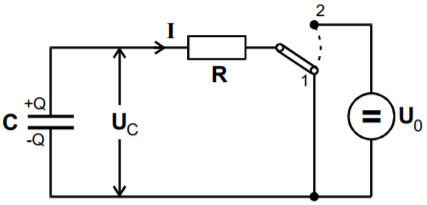
\includegraphics[height=5cm]{entladung.PNG}
  \caption{Auf- und Entladevorgang eines Kondensators über einen Widerstand \cite{sample}}
  \label{fig:Kondensator}
\end{figure}

\subsection{Relaxationsphänomene bei periodisch auftretenden Auslenkungen}
Liegt an einem RC-Kreis eine Wechselspannung $U(t) = U_0 \symup{cos}(\omega t)$ an ist diese
für $\omega \ll \frac{1}{RC}$ ungefähr gleich der Kondensatorspannung. Für größere
Frequenzen entsteht eine Phasenverschiebung $\varphi$ zwischen Auf- und Entladung des Kondensators
über den Widerstand und der Generatorspannung. Die Amplitude $A$ der Kondensatorspannung nimmt ab.


\begin{figure}[H]
  \centering
  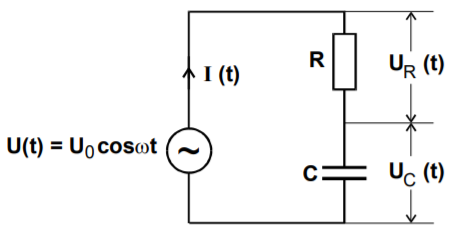
\includegraphics[height=5cm]{wechselspannung.PNG}
  \caption{Wechselspannung in einem RC-Kreis \cite{sample}}
  \label{fig:wechselspannung}
\end{figure}

Um die frequenzabhängige Amplitude und Phasenverschiebung zu ermitteln wird der Ansatz
\begin{equation}
  U_C(t) = A(\omega)\symup{cos}(\omega t + \varphi(\omega))
\end{equation}

gewählt. Mit dem zweiten Kirchhoff'schen Gesetz, Gleichung (3) und $\symup{d}Q = -I\symup{d}t$ folgt:
\begin{equation}
  I(t) = \frac{\symup{d}Q}{\symup{d}t} = C\frac{\symup{d}U_C}{\symup{d}t}
\end{equation}
Aus Gleichung (8) ergibt sich:
\begin{equation}
  U_0 \symup{cos}(\omega t) = -A \omega RC \symup{sin}(\omega t + \varphi) + A(\omega) \symup{cos}(\omega t + \varphi)
\end{equation}
Gleichung (10) muss für alle $t$ erfüllt sein und aus $\omega t = \frac{\pi}{2}$ folgt:
\begin{equation}
  \varphi (\omega) = \symup{arctan} (-\omega RC).
\end{equation}

Für die Phasenverschiebung und die Amplitude lässt sich daraus herleiten:
\begin{align}
  \symup{sin}(\varphi) &= \frac{\omega RC}{\sqrt{1 + \omega^2 R^2C^2}} \\
  A(\omega) &= \frac{U_0}{\sqrt{1 + \omega^2 R^2C^2}}
\end{align}

Die Gleichungen zeigen, dass für kleine Frequenzen die Phasenverschiebung gegen Null und die Amplitude
gegen $U_0$ geht. Für größere Frequenzen wird entstehen Phasenverschiebung und die Amplitude wird kleiner.

\subsection{RC-Kreis als Integrator}
Der RC-Kreis kann unter bestimmten Voraussetzungen eine Spannung, gemäß Abbildung 2, integrieren.
Die Kondensatorspannung $U_C$ ist für hinreichend große Frequenzen $\omega \gg \frac{1}{RC}$ proportional
zu $\int U(t) \: \symup{d}t$.

Mit $|U_C| << |I(t)R|$ und $|U_C| << |U|$ gilt:
\begin{equation}
  U_C(t) = \frac{1}{RC} \int_{0}^{t} U(t') \: \symup{d}t'
\end{equation}
